\section{NGUYÊN HÀM}
\subsection{LÝ THUYẾT CẦN NHỚ}
\subsubsection{Khái niệm nguyên hàm}
\indam{Định nghĩa:}
	\begin{boxdn}
	\begin{itemize}
		\item Cho hàm số $y=f(x)$ xác định trên $K$. Hàm số $F(x)$ được gọi là \textbf{nguyên hàm} của hàm số $f(x)$ trên $K$ nếu $F'(x)=f(x)$ với mọi $x$ thuộc $K$.
		\item Giả sử hàm số $F(x)$ là một nguyên hàm của hàm số $f(x)$ trên $K$. Khi đó
	\begin{itemize}
		\item Với mỗi hằng số $C$, hàm số $G(x)=F(x)+C$ cũng là một nguyên hàm của hàm số $f(x)$ trên $K$.
		\item Ngược lại, với mỗi nguyên hàm $H(x)$ của hàm số $f(x)$ trên $K$ thì tồn tại hằng số $C$ sao cho $H(x)=F(x)+C$ với mọi $x$ thuộc $K$.
	\end{itemize}
	\item Họ (hay tập hợp) tất cả các nguyên hàm của hàm số $f(x)$ trên $K$ được kí hiệu là $\displaystyle\int\limits f(x) \mathrm{~d}x$.
	\end{itemize}
	\end{boxdn}
	
\begin{khung4}{Nhận xét}
\begin{itemize}
	\item Nếu $F(x)$ là một nguyên hàm của hàm số $f(x)$ trên $K$ thì mọi nguyên hàm của hàm số $f(x)$ trên $K$ đều có dạng $F(x)+C$ với $C$ là một hằng số.\\
	Vì vậy, $\displaystyle\int\limits f(x) \mathrm{~d}x=F(x)+C$.
	\item Mọi hàm số liên tục trên $K$ đều có nguyên hàm trên $K$.
	\item $\displaystyle\int\limits f'(x) \mathrm{~d}x=f(x)+C$.
	\item $\displaystyle\int\limits 0 \mathrm{~d}x=C$ và khi quy ước $\displaystyle\int\limits 1 \mathrm{~d}x=\displaystyle\int\limits  \mathrm{~d}x$, ta có $\displaystyle\int\limits  \mathrm{~d}x=x+C$.
\end{itemize}
\textbf{Chú ý:} Biểu thức $f(x)\mathrm{~d}x$ gọi là \textbf{vi phân} của nguyên hàm $F(x)$, kí hiệu là $\mathrm{~d}F(x)$. Vậy
\[\mathrm{~d}F(x)=F'(x)\mathrm{~d}x=f(x)\mathrm{~d}x.\]
\end{khung4}
\subsubsection{Nguyên hàm của một số hàm sơ cấp}
\begin{itemize}
	\item \textbf{Nguyên hàm của hàm số lũy thừa}
	\begin{khung4}{}
	\begin{itemize}
	\item $\displaystyle\int\limits 0 \mathrm{~d}x=C$;
	\item $\displaystyle\int\limits 1 \mathrm{~d}x=x+C$;
	\item $\displaystyle\int\limits x^\alpha \mathrm{~d}x=\dfrac{x^{\alpha+1}}{\alpha+1}+C$ $(\alpha\neq-1)$.
	\end{itemize}
	\end{khung4}
\item \textbf{Nguyên hàm của hàm số $\dfrac{1}{x}$}
\begin{khung4}{}
$\displaystyle\int\limits \dfrac{1}{x} \mathrm{~d}x=\ln|x|+C$.
\end{khung4}
\item \textbf{Nguyên hàm của một số hàm số lượng giác}
\begin{khung4}{}
\begin{itemize}
	\item $\displaystyle\int\limits \cos x \mathrm{~d}x=\sin x+C$;
	\item $\displaystyle\int\limits \sin x \mathrm{~d}x=-\cos x+C$;
	\item $\displaystyle\int\limits \dfrac{1}{\cos^2x} \mathrm{~d}x=\tan x+C$;
	\item $\displaystyle\int\limits \dfrac{1}{\sin^2x} \mathrm{~d}x=-\cot x +C$.
\end{itemize}
\end{khung4}
\item \textbf{Nguyên hàm của hàm số mũ}
\begin{khung4}{}
	\begin{itemize}
		\item $\displaystyle\int\limits \mathrm{e}^x \mathrm{~d}x=\mathrm{e}^x+C$;
		\item $\displaystyle\int\limits \mathrm{a}^x \mathrm{~d}x=\dfrac{\mathrm{a}^x}{\ln \mathrm{a}}+C$ $(a > 0, a\neq 1)$.
	\end{itemize}
\end{khung4}
\end{itemize}
\subsubsection{Tính chất của nguyên hàm}
Cho các hàm số $y=f(x)$, $y=g(x)$ liên tục trên $K$.
\begin{itemize}
	\item $\displaystyle\int\limits kf(x) \mathrm{~d}x=k\displaystyle\int\limits f(x) \mathrm{~d}x$ với $k\in \mathbb{R}$, $k\neq 0$.
	\item $\displaystyle\int\limits\left[f(x)+g(x)\right] \mathrm{~d}x=\displaystyle\int\limits f(x) \mathrm{~d}x+\displaystyle\int\limits g(x) \mathrm{~d}x$.
	\item $\displaystyle\int\limits \left[f(x)-g(x)\right] \mathrm{~d}x=\displaystyle\int\limits f(x) \mathrm{~d}x-\displaystyle\int\limits g(x) \mathrm{~d}x$.
	\item $\left(\displaystyle\int\limits f(x) \mathrm{~d}x\right)'=f(x)$.
\end{itemize}

%-------------------------------------------------------------------------------------------------------------
\subsection{PHÂN LOẠI VÀ PHƯƠNG PHÁP GIẢI TOÁN}
\begin{dang}{Kiểm tra một hàm số là nguyên hàm của hàm số cho trước}
	\textit{Phương pháp: Sử dụng khái niệm nguyên hàm}.
\end{dang}
\begin{vd}%[2D4N1-2]%[Dự án đề cương 3 khối NH24-25 - Đợt 1 - Lê Phúc]
Hàm số $F(x)=x^2+x+1$ có là một nguyên hàm của hàm số $f(x)=2x+1$ trên $\mathbb{R}$ hay không? Vì sao?
\loigiai{
Ta có $F'(x)=(x^2+x+1)'=2x+1$.\\
Suy ra $F'(x)=f(x)$ với mọi $x$ thuộc $\mathbb{R}$.\\
Vậy $F(x)=x^2+x+1$ là một nguyên hàm của hàm số $f(x)=2x+1$ trên $\mathbb{R}$.}
\end{vd}
\begin{vd}%[2D4H1-4]%[Dự án đề cương 3 khối NH24-25 - Đợt 1 - Lê Phúc]
	Hàm số $F(x)=x\ln x$ có là một nguyên hàm của hàm số $f(x)=1+\ln x$ trên $(0;+\infty)$ hay không? Vì sao?
\loigiai{
	Với mọi $x\in (0;+\infty)$ ta có  $F'(x)=(x\ln x)'=\ln x + x\cdot\dfrac{1}{x} = \ln x+1$.\\
	Suy ra $F'(x)=f(x)$ với mọi $x$ thuộc $(0;+\infty)$.\\
	Vậy $F(x)=x\ln x$ có là một nguyên hàm của hàm số $f(x)=1+\ln x$ trên $(0;+\infty)$.}
\end{vd}

\begin{vd}%[2D4V1-4]%[Dự án đề cương 3 khối NH24-25 - Đợt 1 - Lê Phúc]
Hàm số $F(x)=\dfrac{2x^2+x-1}{\mathrm{e}^x}$ có là một nguyên hàm của hàm số $ f(x)=\dfrac{2x^2-5x}{\mathrm{e}^x}$ trên $ \mathbb{R}$ hay không? Vì sao?
	\loigiai{
		Ta có
	\begin{eqnarray*}
	F'(x)&=&\left(\dfrac{2x^2+x-1}{\mathrm{\mathrm{e}}^x}\right)'\\
	&=&\dfrac{\left(2x^2+x-1\right)'\cdot \mathrm{e}^x-\left(\mathrm{e}^x\right)'\cdot\left(2x^2+x-1\right)}{\left(\mathrm{e}^x\right)^2}\\
	&=&\dfrac{(4x+1)\cdot \mathrm{e}^x-\mathrm{e}^x\cdot\left(2x^2+x-1\right)}{\left(\mathrm{e}^x\right)^2}\\
	&=&\dfrac{\mathrm{e}^x\cdot\left(-2x^2+3x+2\right)}{\mathrm{e}^{2x}}\\
	&=&\dfrac{-2x^2+3x+2}{\mathrm{e}^x}\\
	&\neq& f(x).
	\end{eqnarray*} 
	Vậy hàm số $F(x)=\dfrac{2x^2+x-1}{\mathrm{e}^x}$ không là một nguyên hàm của hàm số $ f(x)=\dfrac{2x^2-5x}{\mathrm{e}^x}$ trên $ \mathbb{R}$.
	}
\end{vd}

\begin{dang}{Tìm nguyên hàm của một hàm số}
	\textit{Phương pháp: Sử dụng công thức $\displaystyle\int\limits F'(x) \mathrm{~d}x=F(x)+C$ với $F(x)$ là hàm số có đạo hàm liên tục và các tính chất của nguyên hàm}.
\end{dang}
\setcounter{vd}{0}
\begin{vd}%[2D4N1-2]%[2D4N1-3]%[2D4N1-4]%[Dự án đề cương 3 khối NH24-25 - Đợt 1 - Lê Phúc]
	Tìm nguyên hàm của các hàm số sau
	\begin{multicols}{3}
		\begin{enumerate}
			\item $x^4$.
			\item $\cos x-\sin x$.
			\item $\mathrm{e}^x+\dfrac{1}{x}$.
		\end{enumerate}
	\end{multicols}
	\loigiai{
	\begin{enumerate}
		\item $\displaystyle\int\limits x^4 \mathrm{~d}x=\dfrac{1}{5}x^5+C$.
		\item $\displaystyle\int\limits(\cos x-\sin x) \mathrm{~d}x=\displaystyle\int\limits\cos x \mathrm{~d}x-\displaystyle\int\limits\sin x \mathrm{~d}x=\sin x+\cos x+C$.
		\item $\displaystyle\int\limits\left(\mathrm{e}^x+\dfrac{1}{x}\right) \mathrm{~d}x=\displaystyle\int\limits\mathrm{e}^x \mathrm{~d}x+\displaystyle\int\limits\dfrac{1}{x} \mathrm{~d}x=\mathrm{e}^x+\ln|x|+C$.
	\end{enumerate}
	}
\end{vd}
\begin{vd}%[2D4H1-2]%[Dự án đề cương 3 khối NH24-25 - Đợt 1 - Lê Phúc]
	Tìm nguyên hàm $F(x)$ của hàm số $f(x)=2x+3x^2$ biết $F(0)=1$.
	\loigiai{
	Ta có $\displaystyle\int\limits(2x+3x^2) \mathrm{~d}x=\displaystyle\int\limits2x \mathrm{~d}x+\displaystyle\int\limits3x^2 \mathrm{~d}x=x^2+x^3+C$.\\
	Vì $F(0)=1$ nên $0^2+0^3+C=1$.\\
	Suy ra $C=1$.\\
	Vậy $F(x)=x^2+x^3+1$.
	}
\end{vd}
\begin{vd}%[2D4H1-2]%[Dự án đề cương 3 khối NH24-25 - Đợt 1 - Lê Phúc]
	Cho $F(x)$ là nguyên hàm của hàm số $f(x)=\dfrac{1}{x}$ và $F(1)=5$. Tính $F(3)$.
	\loigiai{
	$F(x)=\displaystyle\int f(x) \mathrm{~d}x=\displaystyle\int \dfrac{1}{x} \mathrm{~d}x=\ln|x|+C$.\\
	Mà $F(1)=5$ nên $C=5$.\\
	Vậy $F(x)=\ln|x|+5$.\\
	Do đó $F(3)=\ln3 +5$.
	}
\end{vd}
\begin{dang}{Ứng dụng}
	\textit{Phương pháp: Mô hình các bài toán thực tiễn thành các bài toán về nguyên hàm}.
\end{dang}
\setcounter{vd}{0}
\begin{vd}%[2D4V1-6]%[Dự án đề cương 3 khối NH24-25 - Đợt 1 - Lê Phúc]
	Một vườn ươm cây cảnh bán một cây sau $6$ năm trồng và uốn tạo dáng. Tốc độ tăng trưởng của cây đó trong suốt 6 năm được tính xấp xỉ bởi công thức $h'(t)=1{,}5 t+5$, trong đó $h(t)$ (cm) là chiều cao của cây sau $t$ (năm). 
	\begin{flushright}
		\textit{(Nguồn: R. Larson and B. Edwards, Calculus 10e, Cengage $2014$).}
	\end{flushright}
	Cây con khi được trồng cao $12$ cm. Tính chiều cao của cây đó sau $6$ năm.
	\loigiai{
	Ta có $h(t)$ là một nguyên hàm của hàm số $h'(t)=1{,}5 t+5$.\\
	Vì $\displaystyle\int\limits (1{,}5t+5) \mathrm{~d}t=\displaystyle\int\limits 1{,}5t \mathrm{~d}t+\displaystyle\int\limits 5 \mathrm{~d}t=\frac{3}{4} \displaystyle\int\limits 2t \mathrm{~d}t+5 \displaystyle\int\limits  \mathrm{~d}t=\frac{3}{4} t^2+5t+C$.\\ 
	Suy ra $h(t)=\frac{3}{4} t^2+5 t+C$.\\
	Vì cây con khi được trồng cao 12 cm nên $h(0)=12$, suy ra $C=12$.\\
	Vậy $h(t)=\dfrac{3}{4} t^2+5 t+12$.\\
	Sau 6 năm, chiều cao của cây đó là \[h(6)=\dfrac{3}{4} \cdot 6^{2}+5 \cdot 6+12=69 \ \text{(cm)}.\]}
\end{vd}
\begin{vd}%[2D4V1-6]%[Dự án đề cương 3 khối NH24-25 - Đợt 1 - Lê Phúc]
	Đối với các dự án xây dựng, chi phí nhân công lao động được tính theo số ngày công. Gọi $m(t)$ là số lượng công nhân được sử dụng ở ngày thứ $t$ (kể từ khi khởi công dự án). Gọi $M(t)$ là số ngày công được tính đến hết ngày thứ $t$ (kể từ khi khởi công dự án). Trong kinh tế xây dựng, người ta đã biết rằng $M'(t)=m(t)$.\\
	Một công trình xây dựng dự kiến hoàn thành trong 400 ngày. Số lượng công nhân được sử dụng cho bởi hàm số $m(t)=800-2 t$, trong đó $t$ tính theo ngày $(0 \le t \le 400)$, $m(t)$ tính theo người.
	\begin{flushright}
	\textit{(Nguồn: A. Bigalke et al., Mathematik, Grundkurs ma-1, Cornelsen $2016$).}
	\end{flushright}
	Đơn giá cho một ngày công lao động là $400\,000$ đồng. Hỏi chi phí nhân công lao động của công trình đó (cho đến lúc hoàn thành) là bao nhiêu đồng?
	\loigiai{
	Vì $M'(t)=m(t)$ nên ta có $M(t)$ là một nguyên hàm của hàm số $m(t)=800-2 t$.\\
	Do $\displaystyle\int\limits (800-2 t) \mathrm{~d}t =800 \displaystyle\int\limits \mathrm{~d}t-\displaystyle\int\limits 2t \mathrm{~d}t=800 t-t^2+C$\\
	nên $M(t)=800 t-t^{2}+C$ với $0 \le t \le 400$. \\
	Vì $M(0)=0$ nên $C=0$.\\ 
	Vậy $M(t)=800 t-t^{2}$.\\
	Số ngày công được tính đến hết ngày thứ $400$ là
	\[M(400)=800\cdot400-400^{2}=160\,000.\]
	Chi phí nhân công lao động của công trình đó (cho đến lúc hoàn thành) là
	\[400\,000\cdot 160\,000=64\,000\,000\,000\ \text{(đồng)}.\]
 }
\end{vd}

\begin{vd}%[2D4C1-6]%[Dự án đề cương 3 khối NH24-25 - Đợt 1 - Lê Phúc]
	Tại một lễ hội dân gian, tốc độ thay đổi lượng khách tham dự được biểu diễn bằng hàm số $B'(t)=20 t^3-300 t^2+1\,000 t$, trong đó $t$ tính bằng giờ $(0 \le t \le 15)$, $B'(t)$ tính bằng khách/giờ.
	\begin{flushright}
	\textit{(Nguồn: A. Bigalke et al., Mathematik, Grundkurs ma-1, Cornelsen 2016),}
	\end{flushright}
	Sau một giờ, $500$ người đã có mặt tại lễ hội.
	\begin{enumerate}
	\item Viết công thức của hàm số $B(t)$ biểu diễn số lượng khách tham dự lễ hội với $0 \le t \le 15$.
	\item Sau $3$ giờ sẽ có bao nhiêu khách tham dự lễ hội?
	\item Số lượng khách tham dự lễ hội lớn nhất là bao nhiêu?
	\item Tại thời điểm nào thì tốc độ thay đổi lượng khách tham dự lễ hội là lớn nhất?
	\end{enumerate}
	\loigiai{
	\begin{enumerate}
		\item Ta có $B(t)$ là một nguyên hàm của hàm số $B'(t)=20 t^3-300 t^2+1\,000 t$.\\
		Ta có $\displaystyle\int\limits(20t^3-300t^2+1\,000t) \mathrm{~d}t=5 \displaystyle\int\limits4t^3 \mathrm{~d}t-100 \displaystyle\int\limits 3t^2\mathrm{~d}t+500 \displaystyle\int\limits 2t\mathrm{~d}t=5 t^4-100 t^3+500t^2+C$\\
		Suy ra $B(t)=5 t^4-100 t^3+500 t^2+C$.\\
		Vì sau một giờ, $500$ người đã có mặt tại lễ hội nên $B(1)=405+C=500$.\\
		Suy ra $C=95$. \\
		Vậy $B(t)=5t^4-100 t^3+500 t^2+95$ với $0 \le t \le 15$.
		\item Số khách tham dự lễ hội sau 3 giờ là
		\[
		B(3)=5 \cdot 3^4-100 \cdot 3^3+500 \cdot 3^2+95=2\,300 \ \text{ (khách).}\]
		\item Ta tìm giá trị lớn nhất của hàm số $B(t)$ trên đoạn $[0;15]$. Ta có
		\[B'(t)=20 t^{3}-300 t^{2}+1\,000 t=20 t\left(t^{2}-15 t+50\right)=20 t(t-5)(t-10).\]	
		Suy ra $B'(t)=0\Leftrightarrow\hoac{&t=0\\&t=5\\&t=10.}$\\
		Ta có $B(0)=95$, $B(5)=3\,220$, $B(10)=95$, $B(15)=28\,220$.\\
		Khi đó, giá trị lớn nhất của hàm số $B(t)$ trên đoạn $[0;15]$ bằng $28\,220$ tại $t=15$.\\
		Vậy số lượng khách tham dự lễ hội lớn nhất là $28\,220$ khách sau $15$ giờ.
		\item Ta tìm $t$ để hàm số $B'(t)$ đạt giá trị lớn nhất trên đoạn $[0 ; 15]$.\\
		Ta có $B''(t)=60 t^2-600 t+1000$. \\
		Suy ra $B''(t)=0\Leftrightarrow\hoac{&t=\dfrac{15-5\sqrt{3}}{3}\\&t=\dfrac{15+5\sqrt{3}}{3}.}$\\
		Ta có $B'(0)=0$; $B'\left(\dfrac{15-5 \sqrt{3}}{3}\right) \approx 962{,}25$;  $B'\left(\dfrac{15+5 \sqrt{3}}{3}\right) \approx -962{,}25$; $B'(15)=15\,000$.\\
		Khi đó, giá trị lớn nhất của hàm số $B'(t)$ trên đoạn $[0;15]$ bằng $15\,000$ tại $t=15$.\\
		Vậy tốc độ thay đổi lượng khách tham dự lễ hội là lớn nhất tại thời điểm $15$ giờ.
	\end{enumerate}
	}
\end{vd}
%-----------------------------------------------------------------------------
\subsection{Bài tập rèn luyện}
\ind{PHẦN I.} \inden{Câu trắc nghiệm nhiều phương án lựa chọn. Mỗi câu hỏi học sinh chỉ chọn một phương án.}\\
\setcounter{ex}{0}
\Opensolutionfile{ans}[ans/2D4-Bai1-TN]%--Đặt tên 2D1-Bai1-Dang1-TN
\begin{ex}%[2D4N1-1]%[Dự án đề cương 3 khối NH24-25 - Đợt 1 - Lê Phúc]
	(\textit{Trích đề thi GKII - THPT Thuận Thành 1-2-3 - Năm học 2024-2025})\\
	Cho hàm số $y=f(x)$ có đạo hàm liên tục trên $\mathbb{R}$. Khẳng định nào sau đây đúng?
	\choice
	{$\displaystyle\int\limits f(x) \mathrm{~d} x=f'(x)+C$, $C \in \mathbb{R}$}
	{$\displaystyle\int\limits f'(x) \mathrm{~d} x=f'(x)+C$, $C \in \mathbb{R}$}
	{$\displaystyle\int\limits f(x) \mathrm{~d} x=\dfrac{1}{2} f^2(x)+C$, $C \in \mathbb{R}$}
	{\True $\displaystyle\int\limits f'(x) \mathrm{~d} x=f(x)+C$, $C \in \mathbb{R}$}
	\loigiai{
		Theo tính chất của nguyên hàm ta có $\displaystyle\int\limits f'(x) \mathrm{~d} x=f(x)+C$, $C \in \mathbb{R}$.
	}
\end{ex}
\begin{ex}%[2D4N1-1]%[Dự án đề cương 3 khối NH24-25 - Đợt 1 - Lê Phúc]
		(\textit{Trích đề thi GKII - THPT Nguyễn Trung Thiện - Năm học 2024-2025})\\
	Cho hàm số $f(x)$ liên tục trên $\mathbb{R}$. Mệnh đề nào dưới đây đúng?
	\choice
	{$\displaystyle\int 5f(x)\mathrm{\,d}x=\displaystyle\int f(x)\mathrm{\,d}x$}
	{$\displaystyle\int 5f(x)\mathrm{\,d}x = \dfrac{1}{5}\int f(x)\mathrm{\,d}x$}
	{\True $\displaystyle\int 5f(x)\mathrm{\,d}x = 5\displaystyle\int f(x)\mathrm{\,d}x$}
	{$\displaystyle\int 5f(x)\mathrm{\,d}x = 5 + \displaystyle\int f(x)\mathrm{\,d}x$}
	\loigiai{
		Ta có $\displaystyle\int 5f(x)\mathrm{\,d}x = 5\displaystyle\int f(x)\mathrm{\,d}x$.
	}
\end{ex}
\begin{ex}%[2D4N1-1]%[Dự án đề cương 3 khối NH24-25 - Đợt 1 - Lê Phúc]
	(\textit{Trích đề thi GKII - THPT An Lương Đông - Năm học 2024-2025})\\
	Cho hàm số $f(x)$ và $y = g(x)$ liên tục trên $\mathbb{R}$. Mệnh đề nào sau đây \textbf{sai}?
	\choice
	{$\displaystyle\int\left[f(x) + g(x)\right]\mathrm{\,d}x = \displaystyle\int f(x)\mathrm{\,d}x + \displaystyle\int g(x)\mathrm{\,d}x$}
	{$\displaystyle\int \left[f(x) - g(x)\right]\mathrm{\,d}x = \displaystyle\int f(x)\mathrm{\,d}x - \displaystyle\int g(x)\mathrm{\,d}x$}
	{\True $\displaystyle\int kf(x)\mathrm{\,d}x = k\displaystyle\int f(x)\mathrm{\,d}x$, với mọi hằng số $k$}
	{$\displaystyle\int \mathrm{d}x = x + C$}
	\loigiai{
		Ta có $\displaystyle\int kf(x)\mathrm{\,d}x = k\displaystyle\int f(x)\mathrm{\,d}x$, với mọi hằng số $k\neq0$.  
	}
\end{ex}
\begin{ex}%[2D4H1-1]%[Dự án đề cương 3 khối NH24-25 - Đợt 1 - Lê Phúc]
		(\textit{Trích đề thi GKII - THPT Phan Bội Châu - Năm học 2024-2025})\\
	Cho hai hàm số $f(x)$ và $g(x)$ liên tục trên $K$ ($K$ là khoảng hoặc đoạn hoặc nửa khoảng của $\mathbb{R}$). Khẳng định nào sau đây là \textbf{sai}?
	\choice
	{\True Nếu $F(x)$ và $G(x)$ đều là nguyên hàm của hàm số $f(x)$ thì $F(x)=G(x)$}
	{Nếu $\displaystyle\int f(x) \mathrm{\,d}x=F(x)+C$ thì $\displaystyle\int f(u) \mathrm{\,d}u=F(u)+C$}
	{$\displaystyle\int kf(x) \mathrm{\,d}x=k \displaystyle\int f(x) \mathrm{\,d}x$ ($k$ là hằng số và $k \neq 0$)}
	{$\displaystyle\int[f(x)-g(x)] \mathrm{\,d}x=\displaystyle\int f(x) \mathrm{\,d}x-\displaystyle\int g(x) \mathrm{\,d}x$}
	\loigiai{
		Các hàm số $F(x)=\dfrac{x^3}{3}+1$ và $G(x)=\dfrac{x^3}{3}+2$ đều là nguyên hàm của hàm số $y=f(x)=x^2$ nhưng $F(x)\ne G(x)$.
	}
\end{ex}
\begin{ex}%[2D4N1-4]%[Dự án đề cương 3 khối NH24-25 - Đợt 1 - Lê Phúc]
	(\textit{Trích đề thi GKII - THPT Thuận Thành 1-2-3 - Năm học 2024-2025})\\
	Họ nguyên hàm của hàm số $y=3^x$ là
	\choice
	{\True $\displaystyle\int\limits 3^x \mathrm{~d} x=\dfrac{3^x}{\ln 3}+C$}
	{$\displaystyle\int\limits 3^x \mathrm{~d} x=3^x\cdot\ln 3+C$}
	{$\displaystyle\int\limits 3^x \mathrm{~d} x=\dfrac{3^x}{x+1}+C$}
	{$\displaystyle\int\limits 3^x \mathrm{~d} x=3^x+C$}
	\loigiai{
		Ta có
		$\displaystyle\int\limits 3^x \mathrm{~d} x=\dfrac{3^x}{\ln 3}+C$.
	}
\end{ex}
\begin{ex}%[2D4N1-2]%[Dự án đề cương 3 khối NH24-25 - Đợt 1 - Lê Phúc]
	(\textit{Trích đề thi GKII - THPT An Lương Đông - Năm học 2024-2025})\\
	Trong các hàm số sau, hàm số nào \textbf{không phải} là nguyên hàm của $f(x) = x^3$?
	\choice
	{$\dfrac{x^4}{4} - 1$}
	{$\dfrac{x^4}{4}$}
	{$\dfrac{x^4}{4}+1$}
	{\True $3x^2$}
	\loigiai{
		Ta thấy $\left(3x^2\right)'=6x$.\\
		Suy ra $3x^2$ không phải là nguyên hàm của $f(x) = x^3$.
	}
\end{ex}
\begin{ex}%[2D4N1-4]%[Dự án đề cương 3 khối NH24-25 - Đợt 1 - Lê Phúc]
	(\textit{Trích đề thi GKII - Trường THPT Nguyễn Thái Bình - Năm học 2024-2025})\\
	Cho hàm số $f(x)=\mathrm{e}^x+2$. Khẳng định nào dưới đây là đúng?
	\choice
	{\True $\displaystyle\int f(x)\mathrm{\,d}x=\mathrm{e}^x+2x+C$}
	{$\displaystyle\int f(x)\mathrm{\,d}x=\mathrm{e}^x+C$}
	{$\displaystyle\int f(x)\mathrm{\,d}x=\mathrm{e}^{x-2}+C$}
	{$\displaystyle\int f(x)\mathrm{\,d}x=\mathrm{e}^x-2x+C$}
	\loigiai{
		Ta có $\displaystyle\int f(x)\mathrm{\,d}x=\displaystyle\int (\mathrm{e}^x+2)\mathrm{\,d}x=\mathrm{e}^x+2x+C$.
	}
\end{ex}
\begin{ex}%[2D4N1-3]%[Dự án đề cương 3 khối NH24-25 - Đợt 1 - Lê Phúc]
	(\textit{Trích đề thi GKII - Trường THPT Nguyễn Thái Bình - Năm học 2024-2025})\\
	Cho hàm số $f(x)=\sin x+2^x$. Khẳng định nào dưới đây là đúng?
	\choice
	{$\displaystyle\int f(x)\mathrm{\,d}x=\cos x+2^x\ln2+C$}
	{\True $\displaystyle\int f(x)\mathrm{\,d}x=-\cos x+\dfrac{2^x}{\ln2}+C$}
	{$\displaystyle\int f(x)\mathrm{\,d}x=\cos x+\dfrac{2^x}{\ln2}+C$}
	{$\displaystyle\int f(x)\mathrm{\,d}x=-\cos x+2^x\ln2+C$}
	\loigiai{
		Ta có $\displaystyle\int f(x)\mathrm{\,d}x=\displaystyle\int(\sin x+2^x)\mathrm{\,d}x=-\cos x+\dfrac{2^x}{\ln2}+C$.
	}
\end{ex}
\begin{ex}%[2D4N1-2]%[Dự án đề cương 3 khối NH24-25 - Đợt 1 - Lê Phúc]
		(\textit{Trích đề thi GKII - THPT Trung học thực hành Sư Phạm - Năm học 2024-2025})\\
	Trong các khẳng định sau, khẳng định nào \textbf{sai}?
	\choice
	{\True $\displaystyle\int x^\alpha \mathrm{\,d}x=\dfrac{x^{\alpha+1}}{\alpha+1}+C$}
	{$\displaystyle\int \dfrac{1}{x} \mathrm{\,d}x=\ln |x|+C$}
	{$\displaystyle\int \mathrm{\,d}x=x+C$}
	{$\displaystyle\int 0 \mathrm{\,d}x=C$}
	\loigiai{
		Xét $\displaystyle\int x^\alpha \mathrm{\,d}x=\dfrac{x^{\alpha+1}}{\alpha+1}+C$ với $\alpha = -1$.\\
		Ta có $\displaystyle\int x^{-1} \mathrm{\,d}x=\displaystyle\int \dfrac{1}{x} \mathrm{\,d}x=\ln |x|+C$.\\
		Vậy $\displaystyle\int x^\alpha \mathrm{\,d}x=\dfrac{x^{\alpha+1}}{\alpha+1}+C$ sai với $\alpha = -1$.
	}	
\end{ex}
\begin{ex}%[2D4H1-3]%[Dự án đề cương 3 khối NH24-25 - Đợt 1 - Lê Phúc]
	(\textit{Trích đề thi GKII - THPT An Lương Đông - Năm học 2024-2025})\\
	Tìm nguyên hàm của hàm số $f(x) = 3\cos x + \dfrac{1}{x^2}$ trên $(0; +\infty)$.
	\choice
	{$3\cos x + \ln x + C$}
	{$3\cos x +\dfrac{1}{x}+ C$}
	{$-3\sin x +\dfrac{1}{x}+ C$}
	{\True  $3\sin x -\dfrac{1}{x} +C$}
	\loigiai{
		Ta có $\displaystyle\int \left(3\cos x + \dfrac{1}{x^2}\right) \mathrm{\,d}x=3\sin x -\dfrac{1}{x} +C$. 
	}
\end{ex}
\begin{ex}%[2D4H1-4]%[Dự án đề cương 3 khối NH24-25 - Đợt 1 - Lê Phúc]
	(\textit{Trích đề thi GKII - Trường THPT Thị xã Quảng Trị - Năm học 2024-2025})\\
	Họ nguyên hàm của hàm số $f(x) = \mathrm{e}^{3x}$ là
	\choice
	{$\dfrac{1}{3}\mathrm{e}^x + C$}
	{$3\mathrm{e}^x + C$}
	{$3\mathrm{e}^{3x} + C$}
	{\True $\dfrac{1}{3}\mathrm{e}^{3x} + C$}
	\loigiai{ Ta có $\displaystyle \int \mathrm{e}^{3x} \mathrm{\,d}x=\dfrac{1}{3}\mathrm{e}^{3x} + C$.}
\end{ex}
\begin{ex}%[2D4H1-3]%[Dự án đề cương 3 khối NH24-25 - Đợt 1 - Lê Phúc]
		(\textit{Trích đề thi GKII - Trường THPT Chuyên Lê Quý Đôn - Năm học 2024-2025})\\
	Họ nguyên hàm của hàm số $f(x)=4x^3+\dfrac{1}{\cos ^2x}$ là
	\choice
	{$x^4-\cot x+C$}
	{$x^4+\cot x+C$}
	{\True $x^4+\tan x+C$}
	{$x^4-\tan x+C$}
	\loigiai{
		Ta có $\displaystyle\int\limits f(x) \mathrm{\,d}x=\displaystyle\int\limits \left(4x^3+\dfrac{1}{\cos ^2x}\right)\mathrm{d}x=x^4+\tan x+C$.
	}
\end{ex}
\begin{ex}%[2D4H1-2]%[Dự án đề cương 3 khối NH24-25 - Đợt 1 - Lê Phúc]
		(\textit{Trích đề thi GKII - Trường THPT Ten Lơ Man - Năm học 2024-2025})\\
	Nguyên hàm của hàm số $f(x)=1+\dfrac{3}{x}$ là $F(x)=ax+b\ln|x|+C$. Tìm $I=a+b$?
	\choice
	{\True $I=4$}
	{$I=5$}
	{$I=6$}
	{$I=2$}
	\loigiai{
		Ta có $\displaystyle\int\limits \left(1+\dfrac{3}{x}\right) \mathrm{\,d}x=x+3\ln |x|+C$.\\
		Do đó $a=1$, $b=3$, suy ra $I=a+b=4$.
	}
\end{ex}
\begin{ex}%[2D4H1-2]%[Dự án đề cương 3 khối NH24-25 - Đợt 1 - Lê Phúc]
	(\textit{Trích đề thi GKII - Trường THPT Lê Lợi - Năm học 2024-2025})\\
	Hàm số $F(x)=2x^3-2x+1$ là nguyên hàm của hàm số nào sau đây?
	\choice
	{$f(x)=6x^2-2+C$}
	{$f(x)=\dfrac{1}{2}x^4-x^2+x+C$}
	{\True $f(x)=6x^2-2$}
	{$f(x)=\dfrac{1}{2}x^4-x^2+x$}
	\loigiai
	{Ta có $F(x)=\displaystyle\int f(x) \mathrm{\,d}x \Rightarrow f(x)=F'(x)=\left(2x^3-2x+1\right)'=6x^2-2$.
	}
\end{ex}
\begin{ex}%[2D4H1-2]%[Dự án đề cương 3 khối NH24-25 - Đợt 1 - Lê Phúc]
		(\textit{Trích đề thi GKII - Trường THPT Việt Nam Ba Lan - Năm học 2024-2025})\\
	Hàm số $F(x) = \ln x$ là một nguyên hàm của hàm số nào sau đây trên khoảng $(0;+\infty)$?
	\choice
	{$f(x) = \dfrac{1}{x^2}$}
	{\True $f(x) = \dfrac{1}{x}$}
	{$f(x) = -\dfrac{1}{x}$}
	{$f(x) = -\dfrac{1}{x^2}$}
	\loigiai{
		Vì $F'(x)=(\ln x)'=\dfrac{1}{x}$ nên $F(x) = \ln x$ là một nguyên hàm của hàm số $f(x) = \dfrac{1}{x}$.
	}
\end{ex}
\begin{ex}%[2D4H1-3]%[Dự án đề cương 3 khối NH24-25 - Đợt 1 - Lê Phúc]
			(\textit{Trích đề thi GKII - Trường THPT An Lương Đông - Năm học 2024-2025})\\
	Biết $F(x)$ là một nguyên hàm của hàm số $f(x) = \sin x$ và đồ thị hàm số $y = F(x)$ đi qua điểm $M(0;1)$. Tính $F\left( \dfrac{\pi}{2} \right)$.
	\choice
	{$F\left(\dfrac{\pi}{2} \right) = 1$}
	{\True $F\left(\dfrac{\pi}{2} \right) = 2$}
	{$F\left(\dfrac{\pi}{2} \right) = -1$}
	{$F\left( \dfrac{\pi}{2} \right) = 0$}
	\loigiai{
		Ta có $F(x)=\displaystyle\int \sin x\mathrm{\,d}x=-\cos x+C$.\\ 
		$F(0)=1\Leftrightarrow -\cos 0+C=1\Leftrightarrow C=2$.\\ 
		Do đó $F(x)=-\cos x+2$.\\
		Vậy  $F\left(\dfrac{\pi}{2} \right) = -\cos\dfrac{\pi}{2}+2=2$.  
	}
\end{ex}
\begin{ex}%[2D4H1-2]%[Dự án đề cương 3 khối NH24-25 - Đợt 1 - Lê Phúc]
		(\textit{Trích đề thi GKII - Trường THPT Phan Bội Châu - Năm học 2024-2025})\\
	Cho $F(x)$ là một nguyên hàm của hàm số $f(x)=x^3$. Giá trị của $F(2)-F(0)$ bằng
	\choice
	{\True $4$}
	{$8$}
	{$16$}
	{$1$}
	\loigiai{Ta có $F(x)=\displaystyle\int x^3\mathrm{\,d}x=\dfrac{x^4}{4}+C$.\\
		Suy ra $F(2)-F(0)=\dfrac{2^4}{4}+C-\dfrac{0^4}{4}-C=4$.
	}
\end{ex}
\begin{ex}%[2D4H1-2]%[Dự án đề cương 3 khối NH24-25 - Đợt 1 - Lê Phúc]
		(\textit{Trích đề thi GKII - Trường THPT Thanh Miện - Năm học 2024-2025})\\
	Hàm số $F(x)$ là một nguyên hàm của hàm số $y = \dfrac{1}{x}$ trên $(-\infty;0)$ thỏa mãn $F(-2) = 0$. Khẳng định nào sau đây đúng?
	\choice
	{\True $F(x) = \ln\left( \dfrac{-x}{2} \right)$ với $x \in (-\infty;0)$}
	{$F(x) = \ln|x| + C$ với $x \in (-\infty;0)$ với $C$ là một số thực bất kì}
	{$F(x) = \ln(-x) + C$ với $x \in (-\infty;0)$ với $C$ là một số thực bất kì}
	{$F(x) = \ln|x| + \ln 2$ với $x \in (-\infty;0)$}
	\loigiai{
 $F(x) = \displaystyle\int \dfrac{1}{x}\mathrm{\,d}x=\ln|x|+C=\ln(-x)+C$ (Do $x\in (-\infty;0)$).  \\
		Ta có $F(-2) = \ln 2 + C = 0 \Rightarrow C = -\ln 2$.  \\
		Vậy $F(x) = \ln(-x) - \ln 2 = \ln\left( \dfrac{-x}{2} \right)$.
	}
\end{ex}
\begin{ex}%[2D4H1-2]%[Dự án đề cương 3 khối NH24-25 - Đợt 1 - Lê Phúc]
			(\textit{Trích đề thi GKII - Trường THPT Việt Nam Ba Lan - Năm học 2024-2025})\\
	Biết $F(x)$ là một nguyên hàm của $f(x) = \dfrac{1}{x+1}$ và $F(0) = 2$ thì $F(1)$ bằng
	\choice
	{$\ln 2$}
	{$2$}
	{$4$}
	{\True $2 + \ln 2$}
	\loigiai{
		Ta có $F(x)=\displaystyle\int \dfrac{1}{x+1}\mathrm{\,d}x=\ln|x+1|+C$. \\
		Vì $F(0)=2$ nên ta có
		\[\ln 1 + C =2 \Leftrightarrow C=2.\]
		Do đó $F(x)=\ln\left|x+1\right|+2$.\\
		Vậy $F(1)=\ln2+2$.
	}
\end{ex}
\begin{ex}%[2D4H1-3]%[Dự án đề cương 3 khối NH24-25 - Đợt 1 - Lê Phúc]
		(\textit{Trích đề thi GKII - Trường THPT Chuyên Nguyễn Đình Chiểu - Năm học 2024-2025})\\
	Tìm nguyên hàm $F(x)$ của hàm số $f(x)=6x+\sin 3x$, biết $F(0)=\dfrac{2}{3}$.
	\choice[2]
	{$F(x)=3x^2-\dfrac{1}{3}\cos 3x+\dfrac{2}{3}$}
	{$F(x)=3x^2-\dfrac{1}{3}\cos 3x-1$}
	{$F(x)=3x^2+\dfrac{1}{3}\cos 3x+1$}
	{\True $F(x)=3x^2-\dfrac{1}{3}\cos 3x+1$}
	\loigiai{
		\begin{eqnarray*}
		F(x)&=&\displaystyle\int\limits f(x) \mathrm{\,d}x\\
		&=&\displaystyle\int\limits \left(6x+\sin 3x\right)\mathrm{d}x\\
		&=&\displaystyle\int\limits 6x\mathrm{d}x+\displaystyle\int\limits \sin 3x\mathrm{d}x\\
		&=&3x^2-\dfrac{1}{3}\cos 3x+C.
		\end{eqnarray*}
		Ta có $F(0)=\dfrac{2}{3} \Leftrightarrow 0-\dfrac{1}{3}\cdot 1+C=\dfrac{2}{3} \Leftrightarrow C=1$.\\
		Vậy $F(x)=3x^2-\dfrac{1}{3}\cos 3x+1$.
	}
\end{ex}
\Closesolutionfile{ans}
%\indapan{10}{ans/2D4-Bai1-TN}

\ind{PHẦN II.} \inden{Câu trắc nghiệm đúng sai. Trong mỗi ý a), b), c), d) ở mỗi câu, học sinh chọn đúng hoặc sai.}\\
\setcounter{ex}{0}
\Opensolutionfile{ans}[ans/2D4-Bai1-DS]%--Đặt tên 2D1-Bai1-DS
\begin{ex}%[2D4H1-1]%[Dự án đề cương 3 khối NH24-25 - Đợt 1 - Lê Phúc]
	(\textit{Trích đề thi GKII - Trường THPT Nguyễn Thái Bình - Năm học 2024-2025})\\
	Cho hàm số $f(x)$, $g(x)$ liên tục trên $\mathbb{R}$. Biết $F(x)=\sin x$ là một nguyên hàm của $f(x)$.
	\choiceTF
	{\True $\displaystyle\int[f(x)+2g(x)]\mathrm{\,d}x=\displaystyle\int f(x)\mathrm{\,d}x+2\displaystyle\int g(x)\mathrm{\,d}x$}
	{$\displaystyle\int[f(x)\cdot g(x)]\mathrm{\,d}x=\displaystyle\int f(x)\mathrm{\,d}x\cdot\displaystyle\int g(x)\mathrm{\,d}x$}
	{\True $\displaystyle\int\left(f(x)+\mathrm{e}^x\right)\mathrm{\,d}x=\sin x+\mathrm{e}^x+C$}
	{$\displaystyle\int\left(f^2(x)+\sin^2x\right)\mathrm{\,d}x=2x+C$}
	\loigiai{
		Vì $F(x)=\sin x$ là một nguyên hàm của $f(x)$ nên $f(x)=F'(x)=\cos x$.
		\begin{itemchoice}
			\itemch \textbf{Đúng}. Ta có $\displaystyle\int[f(x)+2g(x)]\mathrm{\,d}x=\displaystyle\int f(x)\mathrm{\,d}x+2\displaystyle\int g(x)\mathrm{\,d}x$.
			\itemch \textbf{Sai}. Ta có $\displaystyle\int[f(x)\cdot g(x)]\mathrm{\,d}x\ne \displaystyle\int f(x)\mathrm{\,d}x\cdot\displaystyle\int g(x)\mathrm{\,d}x$.
			\itemch \textbf{Đúng}. $\displaystyle\int\left(f(x)+\mathrm{e}^x\right)\mathrm{\,d}x=\displaystyle\int\left(\cos x+\mathrm{e}^x\right)\mathrm{\,d}x=\displaystyle\int\cos x\mathrm{\,d}x+\displaystyle\int\mathrm{e}^x\mathrm{\,d}x=\displaystyle\int(\sin x)'\mathrm{\,d}x+\displaystyle\int\left(\mathrm{e}^x\right)'\mathrm{\,d}x=\sin x+\mathrm{e}^x+C$.
			\itemch \textbf{Sai}. Ta có $\displaystyle\int\left(f^2(x)+\sin^2x\right)\mathrm{\,d}x=\displaystyle\int\left(\cos^2x+\sin^2x\right)\mathrm{\,d}x=\displaystyle\int\mathrm{\,d}x=\displaystyle\int x'\mathrm{\,d}x=x+C$.
		\end{itemchoice}
	}
\end{ex}
\begin{ex}%[2D4H1-2]%[Dự án đề cương 3 khối NH24-25 - Đợt 1 - Lê Phúc]
	(\textit{Trích đề thi GKII - Trường THPT Ngô Gia Tự - Năm học 2024-2025})\\
	Cho hàm số $f(x)=3x^2+1$. Gọi $F(x)$ là nguyên hàm của $f(x)$ trên $\mathbb{R}$.
	\choiceTF
	{$f'(x)=F(x), \forall x \in \mathbb{R}$}
	{\True $F(x)=x^3+x+C$}
	{\True Biết $F(0)=1$. Giá trị của $F(2)$ bằng 11}
	{\True $\displaystyle\int (f(x)-f'(x))\mathrm{\,d}x= x^3-3x^2+x+C$}
	\loigiai{
		\begin{itemchoice}
			\itemch \textbf{Sai}.
			Ta có $F'(x)=f(x), \forall x \in \mathbb{R}$.
			\itemch \textbf{Đúng}.
			$F(x)=\displaystyle\int f(x)\mathrm{\,d}x= \displaystyle\int (3x^2+1)\mathrm{\,d}x= x^3+x+C$.
			\itemch \textbf{Đúng}.
			$F(0)=1$ nên $0^3+0+C=1\Rightarrow C=1$.\\
			$F(x)=x^3+x+1\Rightarrow F(2)=11$.
			\itemch \textbf{Đúng}.
		\begin{eqnarray*}
		\displaystyle\int (f(x)-f'(x))\mathrm{\,d}x &=&\displaystyle\int (3x^2+1-6x)\mathrm{\,d}x\\
		&=&\displaystyle\int 3x^2\mathrm{\,d}x+\displaystyle\int \mathrm{\,d}x-\displaystyle\int6x\mathrm{\,d}x\\
		&=& x^3+x-3x^2+C.
		\end{eqnarray*}
		\end{itemchoice}
	}
\end{ex}
%%%=============EX_3=============%%%
\begin{ex}%[2D4H1-2]%[Dự án đề cương 3 khối NH24-25 - Đợt 1 - Lê Phúc]
	(\textit{Trích đề thi GKII - Trường THPT Trần Cao Vân- Năm học 2024-2025})\\
	Cho hàm số $f(x)=4x^3-2x$, $\forall x\in \mathbb{R}$. Biết $F(x)$ là nguyên hàm của hàm số $f(x)$.
	\choiceTF
	{\True $F'(x)=4x^3-2x$}
	{\True $\displaystyle\int\limits f(x)\mathrm{\,d}x=x^4-x^2+C$}
	{Một nguyên hàm $F(x)$ của hàm số $f(x)$ thoả mãn $F(0)=1$ là $F(x)=x^4-x^2-1$}
	{Biết $F(0)=1$. Khi đó $F(-1)=-1$}
	\loigiai{\begin{itemchoice}
			\itemch \textbf{Đúng}. Do $F(x)$ là nguyên hàm của hàm số $f(x)$ nên $F'(x)=f(x)=4x^3-2x$.
			\itemch \textbf{Đúng}. Ta có $\displaystyle\int f(x)\mathrm{\,d}x=\displaystyle\int\left(4x^3-2x\right)\mathrm{\,d}x=x^4-x^2+C$.
			\itemch \textbf{Sai}. Do $F(x)$ là nguyên hàm của hàm số $f(x)$ nên $F(x)=\displaystyle\int f(x)\mathrm{\,d}x=x^4-x^2+C$.\\
			Do $F(0)=1$ nên $C=1$, suy ra $F(x)=x^4-x^2+1$.
			\itemch \textbf{Sai}. Do $F(x)$ là nguyên hàm của hàm số $f(x)$ và $F(0)=1$ nên $F(x)=x^4-x^2+1$.\\
			Suy ra $F(-1)=(-1)^4-(-1)^2+1=1$.
	\end{itemchoice}}
\end{ex}
\begin{ex}%[2D4H1-4]%[Dự án đề cương 3 khối NH24-25 - Đợt 1 - Lê Phúc]
	(\textit{Trích đề thi GKII - Trường THPT Phan Bội Châu - Năm học 2024-2025})\\
	Cho hàm số $ f(x)=a\mathrm{e}^{2x}+b $ liên tục trên $\mathbb{R}$ (với $a$, $b\in \mathbb{R}$) và $ F(x)=\dfrac{1}{2}\mathrm{e}^{2x}+2x $ là một nguyên hàm của $f(x)$.
	\choiceTF
	{\True $\displaystyle\int f(x) \mathrm{\, d}x=\dfrac{1}{2}\mathrm{e}^{2x}+2x+C$, với $ C $ là hằng số}
	{\True $ f(x)=\mathrm{e}^{2x}+2$}	
	{\True $ a+b=3 $}
	{Một nguyên hàm $ H(x) $ của $f(x)$ thỏa $ H\left(\dfrac{1}{2} \right)=2-\dfrac{\mathrm{e}}{2}  $ là $ H(x)= \dfrac{1}{2}\mathrm{e}^{2x}+2x+1$}
	\loigiai
	{
		\begin{itemchoice}
			\itemch \textbf{Đúng}. $\displaystyle\int f(x) \mathrm{\, d}x=F(x)+C=\dfrac{1}{2}\mathrm{e}^{2x}+2x+C$, với $ C $ là hằng số.
			\itemch \textbf{Đúng}. $ f(x)=F'(x)= \left(\dfrac{1}{2}\mathrm{e}^{2x}+2x \right)'= \mathrm{e}^{2x}+2$.			
			\itemch \textbf{Đúng}. Ta có $ f(x)=\mathrm{e}^{2x}+2$ suy ra $a=1$, $b=2$ nên $a+b=3$.
			\itemch \textbf{Sai}. Ta có $H(x)= \dfrac{1}{2}\mathrm{e}^{2x}+2x+C$.\\ Vì $ H\left(\dfrac{1}{2} \right)=2-\dfrac{\mathrm{e}}{2}  $ nên $ \dfrac{1}{2}\mathrm{e}+2\cdot\dfrac{1}{2}+C= 2-\dfrac{\mathrm{e}}{2}\Rightarrow C=1-\mathrm{e}$.\\
			Vậy $H(x) = \dfrac{1}{2}\mathrm{e}^{2x}+2x+1-\mathrm{e}$.
		\end{itemchoice}
	}
\end{ex}
\begin{ex}%[2D4V1-6]%[Dự án đề cương 3 khối NH24-25 - Đợt 1 - Lê Phúc]
		(\textit{Trích đề thi GKII - Trường THPT Chuyên Lê Quý Đôn - Năm học 2024-2025})\\
	Một loại thuốc $A$ được tiêm vào bệnh nhân, nồng độ (đơn vị: mg/l) của thuốc trong máu sau $x$ phút (kể từ khi bắt đầu tiêm) được xác định bởi công thức $f(x)=\dfrac{30x}{x^2+4}$. Để đưa ra lời khuyên và cách xử lí phù hợp cho bệnh nhân, người ta cần tính toán một số yếu tố về nồng độ của thuốc trong máu.
	\choiceTF
	{Sau $10$ ngày thì nồng độ thuốc $A$ trong máu nhỏ hơn $0{,}002$ mg/l}
	{\True Nồng độ thuốc trong máu đạt giá trị lớn nhất là $7{,}5$\,mg/l tại thời điểm $2$ phút sau khi tiêm}
	{$F(x)=10\ln \left(x^2+4\right)$ là một nguyên hàm của $f(x)$}
	{\True Nồng độ trung bình của thuốc $A$ (làm tròn đến hàng phần trăm) trong khoảng thời gian $30$ phút từ khi bắt đầu tiêm là $2{,}71$\,mg/l}
	\loigiai{
		\begin{itemchoice}
			\itemch \textbf{Sai}.
			Ta có $10$ ngày = $14\,400$ phút.\\
			Ta tính $f(14\,400)=f(14400)=\dfrac{30 \cdot 14\,400}{14\,400^2+4}\approx 0{,}002083>0{,}002$.
			\itemch \textbf{Đúng}.
			Xét hàm số $f(x)=\dfrac{30x}{x^2+4}$ có $f'(x)=\dfrac{30(-x^2+4)}{\left(x^2+4\right)^2}$.\\
			Ta có $f'(x)=0 \Leftrightarrow -x^2+4=0 \Leftrightarrow \hoac{&x=2 \\ &x=-2.}$\\
			Do $x>0$ nên ta nhận $x=2$, khi đó ta có bảng biến thiên sau
			\begin{center}
				\begin{tikzpicture}[font=\normalsize,t style/.style={style=solid}]
					%dòng khai báo
					\tkzTabInit[nocadre=true,lgt=1.2,espcl=2.5,deltacl=0.5]
					{$x$/0.75,$f'(x)$/0.75, $f(x)$/2}
					{$0$, $2$, $+\infty$}
					%dòng xét dấu của đạo hàm
					\tkzTabLine{,+, 0,-,} % z, t, d, h (h: tô miền);
					%Dòng biến thiên f(x)
					\tkzTabVar{-/{$0$}, +/{$7{,}5$}, -/{$0$}}
				\end{tikzpicture}
			\end{center}
			Vậy nồng độ thuốc trong máu đạt giá trị lớn nhất là $7{,}5$\,mg/l tại thời điểm $2$ phút sau khi tiêm.
			\itemch \textbf{Sai}.
			Xét $F(x)=10\ln \left(x^2+4\right)$, ta tính đạo hàm
			\[
			F'(x)=\left[10\ln (x^2+4)\right]'=\dfrac{20x}{x^2+4} \ne \dfrac{30x}{x^2+4} = f(x).
			\]
			\itemch \textbf{Đúng}.
			Xét $G(x)=15\ln \left(x^2+4\right)$ thì $G'(x)=\left[15\ln (x^2+4)\right]'=\dfrac{30x}{x^2+4}$.\\
			Suy ra $\displaystyle\int f(x) \mathrm{\, d}x=15\ln \left(x^2+4\right)+C$.\\
			Nồng độ trung bình của thuốc $A$ (làm tròn đến hàng phần trăm) trong khoảng thời gian $30$ phút từ khi bắt đầu tiêm là
			\[\dfrac{G(30)-G(0)}{30-0}=\dfrac{15\ln 904+C-15\ln 4-C}{30}\approx 2{,}71 \text{ (mg/l).}\]
		\end{itemchoice}
	}
\end{ex}
\Closesolutionfile{ans}
%\indapan{4}{ans/2D4-Bai1-DS}

\ind{PHẦN III.} \inden{Câu trả lời ngắn}\\
\setcounter{ex}{0}
\Opensolutionfile{ans}[ans/2D4-Bai1-TLN]%--Đặt tên 2D1-Bai1-DS
\begin{ex}%[2D4H1-2]%[Dự án đề cương 3 khối NH24-25 - Đợt 1 - Lê Phúc]
	(\textit{Trích đề thi GKII - Trường THPT Thực hành Sư phạm - Năm học 2024-2025})\\
	Hàm số $y=f(x)$ có đồ thị đi qua điểm $(-1; 4)$ và có đạo hàm $f'(x)=3-2x$ với mọi $x \in \mathbb{R}$. Tính giá trị của $f(5)$.
	\shortans[oly]{$-2$}
	\loigiai{
		Ta có $f(x)=\displaystyle\int f'(x) \mathrm{\,d}x=\displaystyle\int (3-2x) \mathrm{\,d}x=3x-x^2+C$.\\
		Suy ra $f(-1)=4 \Leftrightarrow 3\cdot (-1)-(-1)^2+C = 4 \Leftrightarrow C=8$.\\
		Do đó $f(x)=3x-x^2+8$.\\
		Vậy $f(5)=-2$.
	}
\end{ex}
\begin{ex}%[2D4H1-3]%[Dự án đề cương 3 khối NH24-25 - Đợt 1 - Lê Phúc]
	(\textit{Trích đề thi GKII - Trường THPT Chuyên Lê Quý Đôn - Năm học 2024-2025})\\
	Cho $f(x)=\dfrac{1}{\sin ^2 x}$. Biết rằng $F(x)$ là một nguyên hàm của $f(x)$ thỏa $F\left(\dfrac{\pi}{6}\right)=0$. Tính $F\left(\dfrac{\pi}{3}\right)$. (\textit{Kết quả được làm tròn đến hàng phần trăm})
	\shortans[oly]{$1{,}15$}
	\loigiai{Ta có 
	$F(x)=\displaystyle\int f(x) \mathrm{\,d}x=\displaystyle\int \dfrac{1}{\sin^2{x}} \mathrm{\,d}x=-\cot x+C$.\\
	Mà $F\left(\dfrac{\pi}{6}\right)=0$ nên $C=\sqrt{3}$.\\
	Suy ra $F(x)=-\cot x+\sqrt{3}$.\\
	Vậy $F\left(\dfrac{\pi}{3}\right)=\dfrac{2\sqrt{3}}{3}\approx1{,}15$.
	}
\end{ex}
\begin{ex}%[2D4H1-6]%[Dự án đề cương 3 khối NH24-25 - Đợt 1 - Lê Phúc]
	(\textit{Trích đề thi GKII - Trường THPT Việt Nam Ba Lan - Năm học 2024-2025})\\
	Khi nghiên cứu một quần thể vi khuẩn, người ta nhận thấy quần thể vi khuẩn đó ở ngày thứ $t$ có số lượng $N(t)$ con. Biết rằng tốc độ phát triển của quần thể đó là $N'(t)=\dfrac{8\,000}{t}$ và sau ngày thứ nhất $(t=1)$ có $250$ nghìn con. Số lượng vi khuẩn sau $10$ ngày là bao nhiêu nghìn con (\textit{làm tròn đến hàng đơn vị}).
	\shortans[oly]{$268$}
	\loigiai{
		Ta có $N(\mathrm{t})=\displaystyle\int N'(t) \mathrm{\,d} t=\displaystyle\int \dfrac{8\,000 \mathrm{\,d} t}{t}=8\,000 \ln |t|+C$.\\
		Ngày thứ nhất số lượng vi khuẩn là $250\,000$ con nên $N(1)=250\,000$ con, tức là $C=250\,000$.\\
		Số lượng vi khuẩn sau 10 ngày là
		$ N(10)=8\,000 \cdot \ln |10|+250\,000 \approx 268\,420$ (con) $\approx 268$ (nghìn con).
	}
\end{ex}
\begin{ex}%[2D4V1-6]%[Dự án đề cương 3 khối NH24-25 - Đợt 1 - Lê Phúc]
		(\textit{Trích đề thi GKII - Trường THPT Trần Cao Vân - Năm học 2024-2025})\\
	Một xe ô tô đang chạy với vận tốc $18 \mathrm{~m} / \mathrm{s}$ thì người lái xe bất ngờ phát hiện chướng ngại vật trên đường. Người lái xe phản ứng một giây, sau đó đạp phanh khẩn cấp. Kể từ thời điểm này, ô tô chuyển động chậm dần đều với tốc độ $v(t)=-10 t+20~(\mathrm{m} / \mathrm{s})$, trong đó $t$ là thời gian tính bằng giây kể từ lúc đạp phanh. Hỏi kể từ lúc người lái xe phát hiện chướng ngại vật trên đường đến khi dừng hẳn, ô tô di chuyển được quãng đường bằng bao nhiêu mét?
	\shortans[oly]{$20$}
	\loigiai{
		Ta có ô tô dừng khi $v(t)=0\Leftrightarrow -10 t+20 =0\Leftrightarrow t=2$.\\
		Quãng đường đi được trong $t$ giây là
		\[s(t)=\displaystyle\int v(t) \mathrm{\,d} t=\displaystyle\int\limits (-10t+20) \mathrm{\,d} t=-5t^2+20t+C.\]
	Mà $s(0)=0$ nên $C=0$.\\
	Do đó $s(t)=-5t^2+20t$.\\
	Vậy quãng đường xe di chuyển từ lúc phát hiện chướng ngại vật đến khi dừng hẳn là
	\[s(2)=-5\cdot 2^2+20\cdot 2=20\ (\mathrm{m} / \mathrm{s}).\]
	}
\end{ex}
\begin{ex}%[2D4V1-6]%[Dự án đề cương 3 khối NH24-25 - Đợt 1 - Lê Phúc]
		(\textit{Trích đề thi GKII - Trường THPT Phan Bội Châu - Năm học 2024-2025})\\
	Tại một nhà máy, gọi $C(x)$ là tổng chi phí (tính theo triệu đồng) để sản xuất $x$ tấn sản phẩm A trong một tháng. Khi đó, đạo hàm $C'(x)$ (gọi là chi phí cận biên) cho biết tốc độ tăng tổng chi phí theo lượng sản phẩm được sản xuất. Giả sử chi phí cận biên (tính theo triệu đồng/tấn) của nhà máy được ước lượng bởi công thức $C'(x)=9-0{,}04x+0{,}00021x^2$ với $0\le x\le 104$. Biết rằng $C(0)=20$ (triệu đồng) gọi là chi phí cố định. Tính tổng chi phí khi nhà máy sản xuất $98$ tấn sản phẩm A trong tháng (\textit{làm tròn kết quả đến hàng đơn vị}).
	\shortans[oly]{$776$}
	\loigiai{
		Ta có
		\allowdisplaybreaks
		\begin{eqnarray*}
		C(x)&=&\displaystyle\int\limits C'(x)\mathrm{\,d}x\\
		&=&\displaystyle\int\limits{(9-0{,}04x+0{,}00021x^2)}\mathrm{\,d}x\\
		&=&9x-0{,}02x^2+0{,}00007x^3+C.
		\end{eqnarray*}
	Mà $C(0)=20$ nên $C=20$.\\
	Do đó $C(x)=9x-0{,}02x^2+0{,}00007x^3+20$.\\
	Tổng chi phí khi sản xuất $98$ tấn sản phẩm A là
	\[ C(98)=9\cdot 98-0{,}02\cdot 98^2+0{,}00007\cdot 98^3+20 \approx 776\ \text{(triệu đồng)}.\]
}
\end{ex}
\Closesolutionfile{ans}
%\indapan{6}{ans/2D4-Bai1-TLN}

\ind{PHẦN IV.} \inden{Tự luận.}\\
\setcounter{ex}{0}
\begin{ex}%[2D4H1-2]%[Dự án đề cương 3 khối NH24-25 - Đợt 1 - Lê Phúc]
		(\textit{Trích đề thi GKII - Trường THPT Trần Quang Khải - Năm học 2024-2025})\\
	Cho hàm số $ f(x) = 3x^2 - 2x + 3 $.
	\begin{enumerate}
		\item Tìm tất cả các nguyên hàm của hàm số $ f(x) = 3x^2 - 2x + 3 $ trên $ \mathbb{R} $. 
		\item Tìm nguyên hàm $ F(x) $ của hàm $ f(x) = 3x^2 - 2x + 3 $ trên $ \mathbb{R} $ thoả mãn $ F(0) = 2 $. 
	\end{enumerate}
	\loigiai
	{
		\begin{enumerate}[label=\alph*)] 
			\item Ta có  $F(x) = \displaystyle \int f(x) \mathrm{d}x=\displaystyle \int (3x^2 - 2x + 3)\mathrm{d}x =x^3-x^2+3x+C$. 
			\item Ta có $F(x)=x^3-x^2+3x+C$.\\
			Do $ F(0) = 2 \Leftrightarrow C = 2$ nên $F(x)=x^3-x^2+3x+2$. 
		\end{enumerate}
	}
\end{ex}
\begin{ex}%[2D4H1-3]%[Dự án đề cương 3 khối NH24-25 - Đợt 1 - Lê Phúc]
		(\textit{Trích đề thi GKII - Trường THPT Ten Lơ Man - Năm học 2024-2025})\\
	Cho hàm số $f(x)$ thỏa mãn $f'(x)=5-3\cos x$, $\forall x \in \mathbb{R}$ và $f(0)=-10$. Tìm hàm số $f(x)$.
	\loigiai{
		Ta có $\displaystyle\int f'(x)\mathrm{\,d}x=\displaystyle\int (5-3\cos x)\mathrm{\,d}x=5x-3\sin x+C$.\\
		Suy ra $f(x)=5x-3\sin x+C$ với $C$ là hằng số.\\
		Khi đó $f(0)=-10\Leftrightarrow 5\cdot0-3\sin 0 +C=-10 \Leftrightarrow C=-10$.\\
		Vậy $f(x)=5x-3\sin x-10$.
	}
\end{ex}
\begin{ex}%[2D4H1-2]%[Dự án đề cương 3 khối NH24-25 - Đợt 1 - Lê Phúc]
	Họ nguyên hàm của hàm số $f(x)=3x^2+2x+5$ trên $\mathbb{R}$ là $F(x)=ax^3+bx^2+5x+C$. Giá trị biểu thức $T=a+b$ bằng bao nhiêu?
	\loigiai{
	Ta có $f(x)=F'(x)=\left(ax^3+bx^2+5x+C\right)'=3ax^2+2bx+5$.\\
	Mà $f(x)=3x^2+2x+5$, $\forall x \in \mathbb{R}$ nên
	\[\heva{&3a=3\\&2b=2}\Leftrightarrow \heva{&a=1\\&b=1.}\]
	Vậy $a+b=2$.
	}
\end{ex}
\begin{ex}%[2D4H1-2]%[Dự án đề cương 3 khối NH24-25 - Đợt 1 - Lê Phúc]
	Cho hàm số $y=f(x)$ có đạo hàm liên tục trên $[1;4]$ thỏa mãn $f(1)=4$ và $f'(x)=2x^2+3\sqrt{x}$. Tìm hàm số $f(x)$.
	\loigiai{
	Ta có $f(x)=\displaystyle\int f'(x)\mathrm{\,d}x=\displaystyle\int (2x^2+3\sqrt{x})\mathrm{\,d}x=\dfrac{2}{3}x^3+2\sqrt{x^3}+C$.\\
	Mà $f(1)=4$ nên $C=\dfrac{4}{3}$.\\
	Vậy $f(x)=\dfrac{2}{3}x^3+2\sqrt{x^3}+\dfrac{4}{3}$.
	}
\end{ex}
\begin{ex}%[2D4H1-4]%[Dự án đề cương 3 khối NH24-25 - Đợt 1 - Lê Phúc]
	Biết một nguyên hàm của hàm số $f(x)=x^6+\mathrm{e}^x$ trên $\mathbb{R}$ là $F(x)=\dfrac{x^7}{a}+b\mathrm{e}^x+5$ (với $a$, $b\in \mathbb{Z}$, $a\neq 0$). Tính giá trị của biểu thức $a+b$.
	\loigiai{
		Ta có $F'(x)=\dfrac{7x^6}{a}+b\mathrm{e}^x$.\\
		Vì $F'(x)=f(x)$ nên $\heva{&\dfrac{7}{a}=1\\&b=1}\Leftrightarrow \heva{&a=7\\&b=1.}$\\
		Vậy $a+b=7+1=8$.
	}
\end{ex}
\begin{ex}%[2D4H1-6]%[Dự án đề cương 3 khối NH24-25 - Đợt 1 - Lê Phúc]
	Giả sử lợi nhuận biên của một loại sản phẩm của nhà máy được tính theo công thức $P'(x)=18-0{,}04x$. Trong đó $P(x)$ là lợi nhuận thu được khi bán $x$ tấn sản phẩm ($P(x)$ có đơn vị là triệu đồng). Chêch lệch lợi nhuận khi bán $100$ tấn sản phẩm so với khi bán $50$ tấn sản phẩm là bao nhiêu triệu đồng?
	\loigiai{
		$P(x)=\displaystyle\int P'(x) \mathrm{\,d}x=\displaystyle\int (18-0{,}04x) \mathrm{\,d}x=18x-0{,}02x^2+C$.\\
		Chêch lệch lợi nhuận khi bán $100$ tấn sản phẩm so với khi bán $50$ tấn sản phẩm là
		\[P(100)-P(50)=1\,600+C-850-C=750\ \text{(triệu đồng)}.\]
	} 
\end{ex}

\begin{ex}%[2D4H1-6]%[Dự án đề cương 3 khối NH24-25 - Đợt 1 - Lê Phúc]
	Xét dao động điều hòa của một chất điểm có vận tốc tức thời tại thời điểm $t$ là $v(t)=-0,2\pi\sin(\pi t)$, trong đó $t$ tính bằng giây, $v(t)$ tính bằng $\mathrm{m}/\mathrm{s}$. Tìm phương trình li độ $x(t)$, biết $v(t)$ là đạo hàm của $x(t)$ và $x(0)=0{,}2$ (m).
	\loigiai{
	Vì $v(t)=x'(t)$ nên $x(t)$ là một nguyên hàm của $v(t)$.\\
	Ta có $x(t)=\displaystyle\int-0,2\pi\sin(\pi t)\mathrm{\,d}t=-0,2\pi\displaystyle\int \sin(\pi t)\mathrm{\,d}t=0{,}2\cos(\pi t)+C$.\\
	Vì $x(0)=0{,}2$ nên $C=0$.\\
	Vậy $x(t)=0{,}2\cos(\pi t)$.
	} 
\end{ex}
\begin{ex}%[2D4V1-6]%[Dự án đề cương 3 khối NH24-25 - Đợt 1 - Lê Phúc]
	(\textit{Trích đề thi GKII - Trường THPT Chuyên Nguyễn Đình Chiểu - Năm học 2024-2025})\\
	Một hộ gia đình sản xuất cơ khí nhỏ mỗi ngày sản xuất được $x$ sản phẩm $(0 \le x \le 20)$. Chi phí biên để sản xuất $x$ sản phẩm, tính bằng nghìn đồng, cho bởi hàm số sau $C'(x)=3x^2-4x+10$. Biết rằng chi phí cố định ban đầu để sản xuất là $500$ nghìn đồng. Giả sử cơ sở này bán hết sản phẩm mỗi ngày với giá $270$ nghìn đồng/sản phẩm. Tính lợi nhuận tối đa mà gia đình đó thu được khi sản xuất và bán sản phẩm.
	\loigiai{
		Chi phí để sản xuất $x$ sản phẩm bằng \[C(x)=\displaystyle\int\limits C'(x) \mathrm{\,d}x=x^3-2x^2+10x+C.\]\\
		Mà chi phí cố định ban đầu để sản xuất $500$ nghìn đồng nên suy ra $C(0)=500$.\\
		Khi đó $C(0)=500 \Rightarrow C=500 \Rightarrow C(x)=x^3-2x^2+10x+500$.\\
		Khi bán $x$ sản phẩm, số tiền thu được là $270x$ nghìn đồng.\\
		Do đó lợi nhuận thu được là $T(x)=-x^3+2x^2+260x-500$ (nghìn đồng).\\
		Ta có $T'(x)=-3x^2+4x+260=0 \Leftrightarrow x=10$ hoặc $x=-\dfrac{26}{3}$ (loại).\\
		Bảng biến thiên
		\begin{center}
			\begin{tikzpicture}
				\tkzTabInit[nocadre=true, lgt=1.2, espcl=4, deltacl=0.5]
				{$x$/0.7,$T’(x)$/0.7,$T(x)$/2}
				{$0$,$10$,$20$}
				\tkzTabLine{ ,+,0,-, }
				\tkzTabVar{-/$-500$,+/$1\,300$,-/$-2\,500$}
			\end{tikzpicture}
		\end{center}
		Lợi nhuận tối đa là $1\,300$ nghìn đồng khi sản xuất $10$ sản phẩm mỗi ngày.
	} 
\end{ex}
\begin{ex}%[2D4V1-6]%[Dự án đề cương 3 khối NH24-25 - Đợt 1 - Lê Phúc]
	Mực nước trong hồ chứa của nhà máy thủy điện thay đổi trong suốt một ngày do nước chảy ra khi thủy triều xuống và nước chảy vào khi thủy triều lên. Tốc độ thay đổi của mực nước được xác định bởi hàm số \\$h'(t)=\dfrac{1}{90}\left(t^2-17t+60\right)$, trong đó $t$  tính bằng giờ $(0\le t\le 24)$  và $h'(t)$ tính bằng mét/giờ. Tại thời điểm $t=0$, mực nước trong hồ chứa cao $8$ mét. Hỏi tại thời điểm  $t=6$, mực nước trong hồ chứa cao bao nhiêu mét?
	\loigiai{
	Mực nước trong hồ chứa tại thời điểm $t$ là
	\[h(t)=\displaystyle\int h'(t) \mathrm{\,d}t=\displaystyle\int \dfrac{1}{90}\left(t^2-17t+60\right) \mathrm{\,d}t=\dfrac{1}{90}\left(\dfrac{t^3}{3}-\dfrac{17t^2}{2}+60t\right)+C.\]
	Ta có $h(0)=8\Rightarrow C=8$.\\
	Suy ra $h(t)=\dfrac{1}{90}\left(\dfrac{t^3}{3}-\dfrac{17t^2}{2}+60t\right)+8$.\\
	Tại thời điểm  $t=6$  mực nước trong hồ chứa là
	\[h(6)=\dfrac{1}{90}\left(\dfrac{6^3}{3}-\dfrac{17\cdot 6^2}{2}+60\cdot 6\right)+8=9{,}4\ \text{(m)}.\]
	} 
\end{ex}
\begin{ex}%[2D4C1-6]%[Dự án đề cương 3 khối NH24-25 - Đợt 1 - Lê Phúc]
	(\textit{Trích đề thi GKII - Trường THPT Ngô Quyền - Năm học 2024-2025})\\
	Chủ một trung tâm thương mại muốn cho thuê một số gian hàng như nhau. Người đó muốn tăng giá cho thuê của mỗi gian hàng thêm $x$ (triệu đồng) ($x\geq 0$). Tốc độ thay đổi doanh thu từ các gian hàng đó được biểu diễn bởi hàm số $T' (x)=-20x+300$, trong đó   tính bằng triệu đồng. Biết rằng nếu người đó tăng giá thuê cho mỗi gian hàng thêm $10$ triệu đồng thì doanh thu là $12\,000$ triệu đồng. Doanh thu cao nhất mà người đó có thể thu về là bao nhiêu? (tính bằng chục triệu đồng).
	\loigiai{
		Tốc độ thay đổi doanh thu được cho bởi $ T'(x) = -20x + 300$. Do đó, doanh thu tại thời điểm $x$ là
		\[
		T(x) =\displaystyle\int(-20x + 300)\mathrm{\,d}x= -10x^2 + 300x + C.
		\]
		Với \( x = 10 \), doanh thu \( T(10) = 12000 \) (triệu đồng), ta có
		\allowdisplaybreaks 
		\begin{eqnarray*}
			&& T(10) = -10\cdot 10^2 + 300\cdot10 + C = -1\,000 + 3\,000 + C = 2\,000+C \\
			&\Rightarrow& 12\,000 = 2\,000+C \\
			&\Rightarrow& C  = 10\,000.
		\end{eqnarray*}
		Vậy hàm doanh thu là $T(x) = -10x^2 + 300x + 10\,000$.\\
		Hàm doanh thu là hàm số bậc hai nên đạt doanh thu cao nhất tại  $x=-\dfrac{b}{2a} = \dfrac{300}{2 \cdot 10} = 15$. \\
		Doanh thu cao nhất mà người đó có thể thu về là
		\[
		T(15) = 12\,250 \text{ (triệu đồng)}= 1\,225 \text{ (chục triệu đồng)}.
		\]
	}
\end{ex}

\indapan{10}{ans/2D4-Bai1-TN}
\indapan{4}{ans/2D4-Bai1-DS}
\indapan{6}{ans/2D4-Bai1-TLN}